%%%%%%%%%%%%%%%%%%%%%%%%%%%%%%%%%%%%%%%%%
% FILE UTAMA
% Author: Julio Adisantoso
%
% Isi file ini seharusnya tidak banyak diubah
% kecuali jika ada penambahan file eksternal
%
%%%%%%%%%%%%%%%%%%%%%%%%%%%%%%%%%%%%%%%%%

%-------------------------------------------------------
%	PACKAGES AND OTHER DOCUMENT CONFIGURATIONS
%-------------------------------------------------------
\documentclass[a4paper, 12pt, twoside]{book} % Document font size and equations flushed left
%
% Hyphenation untuk Indonesia 
%
% @author  Andreas Febrian
% @version 1.00
% 
% Tambahkan cara pemenggalan kata-kata yang salah dipenggal secara otomatis 
% oleh LaTeX. Jika kata tersebut dapat dipenggal dengan benar, maka tidak 
% perlu ditambahkan dalam berkas ini. Tanda pemenggalan kata menggunakan 
% tanda '-'; contoh: menarik  --> pemenggalan: me-na-rik
%

\hyphenation{
    % alphabhet A
    a-na-li-sa a-tur ada-lah
    a-pli-ka-si 
    % alphabhet B
    ba-ngun-an 
    be-be-ra-pa 
    ber-ge-rak
    ber-ke-lan-jut-an 
    ber-pe-nga-ruh ber-no-ul-li
    % alphabhet C
    ca-ri
    % alphabhet D
    di-sim-pan di-pim-pin de-ngan da-e-rah di-ba-ngun da-pat di-nya-ta-kan 
    di-sim-bol-kan di-pi-lih di-li-hat de-fi-ni-si di-kem-bang-kan di-be-ri-kan
    % alphabhet E
    e-ner-gi eks-klu-sif
    % alphabhet F
    fa-si-li-tas
    % alphabhet G
    ga-bung-an ge-rak
    % alphabhet H
    ha-lang-an
    % alphabhet I
    % alphabhet J
    jang-krik
    % alphabhet K
    ke-hi-lang-an
    ku-ning 
    kua-li-tas ka-me-ra ke-mung-kin-an ke-se-pa-ham-an
    % alphabhet L
    ling-kung-an
    % alphabhet M
    me-neng-ah
    meng-a-tas-i me-mung-kin-kan me-nge-na-i me-ngi-rim-kan 
    meng-u-bah meng-a-dap-ta-si me-nya-ta-kan mo-di-fi-ka-si
    meng-a-tur meng-um-pul-kan meng-hi-tam-kan
    % alphabhet N
    nya-ta non-eks-klu-sif
    % alphabhet O
    % alphabhet P
	pe-nye-rap-an 
	pe-ngon-trol
    pe-mo-del-an
    pe-ran  pe-ran-an-nya
    pem-ba-ngun-an pre-si-den pe-me-rin-tah prio-ri-tas peng-am-bil-an 
    peng-ga-bung-an pe-nga-was-an pe-ngem-bang-an 
    pe-nga-ruh pa-ra-lel-is-me per-hi-tung-an per-ma-sa-lah-an 
    pen-ca-ri-an peng-struk-tur-an
    % alphabhet Q
    % alphabhet R
    ran-cang-an 
    ring-kas-an
    % alphabhet S
    si-mu-la-si sa-ngat
    % alphabhet T
    te-ngah
    ter-da-pat
    % alphabhet U
    % alphabhet V
    % alphabhet W
    % alphabhet X
    % alphabhet Y
    % alphabhet Z
    % special
}
% ---------------------
% FILE DEFINISI DAN DATA SKRIPSI
% ---------------------

% --- JUDUL DALAM HURUF BESAR
\def\JUDUL {SPAM FILTER MENGGUNAKAN MODEL KLASIFIKASI MULTIVARIATE BERNOULLI DAN MULTINOMIAL NAIVE BAYES}

% --- Judul dalam huruf normal
\def\Judul {Spam Filter Menggunakan Model Klasifikasi Multivariate Bernoulli dan Multinomial Naive Bayes}

% --- Judul dalam bahasa Inggris
\def\Judulen {Spam Filter Using Multivariate Bernoulli Classifiers and Multinomial Naive Bayes Classifiers}

% --- Identitas mahasiswa dan pembimbing
\def\NAMA {DENIS FADILLAH}
\def\Nama {Denis Fadillah}
\def\NIM  {G64124052}

\def\jumlahPembimbing{1}

\def\PEMBIMBING {JULIO ADISANTOSO}
\def\Pembimbing {Ir. Julio Adisantoso, M.Komp}
\def\PembimbingNIP {19620714 198601 1 002}

\def\PEMBIMBINGDUA {ABCD}
\def\PembimbingDua {Abcd}
\def\PembimbingDuaNIP {123456789}

% --- Identitas penguji
\def\pengujisatu {Ahmad Ridha, SKom MS}
\def\pengujidua {Dr Imas Sukaesih Sitanggang, SSi MKom}

% --- Identitas waktu dan Ketua Departemen
\def\tahun {2014}
\def\bulantahun {Desember 2014}
\def\Kadept {Dr.Ir. Agus Buono, MSc}


% ------ BAGIAN DI BAWAH INI JANGAN DIUBAH -----
%
\newcommand{\ttdpembimbing}[1]{%
	\ifthenelse{\equal{#1}{2}}
	{%
		\begin{table*}[h!]
			\begin{tabular}{p{8cm} p{4cm}}
				\underline{\Pembimbing} & \underline{\PembimbingDua}\\
				Pembimbing I & Pembimbing II\\
			\end{tabular}
		\end{table*}
	}%
	{%
		\begin{center}
			\underline{\Pembimbing} \\
			Pembimbing \\
		\end{center}
	}%
}%

\newcommand{\cetakAbstrak}[1]{%
	\ifthenelse{\equal{#1}{2}}
	{\textbf{\PEMBIMBING}~dan \textbf{\PEMBIMBINGDUA}.}
	{\textbf{\PEMBIMBING}.}%
}%
\newcommand{\cetakAbstrakEN}[1]{%
	\ifthenelse{\equal{#1}{2}}
	{\textbf{\PEMBIMBING}~\textit{and} \textbf{\PEMBIMBINGDUA}.}
	{\textbf{\PEMBIMBING}.}%
}%

% -------------------
% Abstrak bahasa Indonesia
% -------------------
\def\abstrakid {%
% -------- awal abstrak -----------
Pertumbuhan pengguna email memicu peningkatan spam email sehingga diperlukan teknik spam filter. Model klasifikasi Naive Bayes (NB) adalah salah satu supervised learning yang dapat digunakan untuk spam filter karena tingkat akurasi yang tinggi dan mudah diimplementasikan. \tm{Multivariat Bernoulli NB} menggunakan atribut Boolean sedangkan Multinomial NB menggunakan frekuensi term, adalah dua model NB yang sering digunakan untuk fungsi klasifikasi. Pemilihan fitur ciri yang baik juga berpengaruh pada peningkatan akurasi klasifikasi. Penelitian ini mencoba memodelkan \tm{spam filter} menggunakan model klasifikasi \tm{Multivariat Bernoulli} dan \tm{Multinomial NB} kemudian membandingkan akurasinya. Seleksi fitur \tm{chi-square} dipilih dengan harapan dapat menghasilkan fitur ciri yang lebih baik. Model \tm{Multinomial NB} tanpa seleksi fitur menghasilkan akurasi tertinggi sebesar 95.31\%, sedangkan untuk tingkat akurasi terendah didapatkan pada model Multivariate Bernoulli tanpa seleksi fitur sebesar 89.69\%. Seleksi fitur chi-square meningkatkan akurasi model Multivariate Bernoulli sebesar 3.31\%, sedangkan \tm{Multinomial NB} mengalami penurunan akurasi sebesar 1.98\%.
% -------- akhir abstrak -----------
}%
% -------------------
% Kata kunci bahasa Indonesia
% -------------------
\def\katakunciid {%
	multinomial, multivariat bernoulli, naive bayes, spam filter
}%

% -------------------
% Abstrak bahasa Inggris
% -------------------
\def\abstraken {%
\tm{%
% -------- awal abstrak ----------
The growth of email users is triggers an increase in spam email, so that the required spam filters. Naive Bayes classification model (NB) is one of the supervised learning that can be used for spam filters because of high accuracy and easy to implement. Multivariate Bernoulli NB that is using Boolean attribute while Multinomial NB is using term frequency, those are two NB models which often used for classification function. Selection of good features will also affects the improvement of classification accuracy. This research is trying to modelling spam filter by using Multivariate Bernoulli and Multinomial NB classifiers then to compare both accuracy outputs. Chi-square feature selection also was chosen to hope producing a better features. Multinomial NB models without feature selection resulted in the highest accuracy of 95.31\%, while the lowest accuracy rate obtained in the Multivariate Bernoulli models without feature selection by 89.69\%. Chi-square feature selection improve the accuracy of the model Multivariate Bernoulli at 3.31\%, while the accuracy of Multinomial NB decreased by 1.98\%.
% -------- akhir abstrak ----------
}%
}%
% -------------------
% Kata kunci bahasa Inggris
% -------------------
\def\katakuncien {%
	multinomial, multivariat bernoulli, naive bayes, spam filter
}%

\usepackage{mathptmx}
\usepackage{xcolor,colortbl}
\usepackage{multicol}
\usepackage{multirow}
\usepackage{array}
\newcolumntype{L}[1]{>{\raggedright\let\newline\\\arraybackslash\hspace{0pt}}m{#1}}
\newcolumntype{C}[1]{>{\centering\let\newline\\\arraybackslash\hspace{0pt}}m{#1}}
\newcolumntype{R}[1]{>{\raggedleft\let\newline\\\arraybackslash\hspace{0pt}}m{#1}}
\usepackage[hidelinks=true]{hyperref}
\usepackage[hyphenbreaks]{breakurl}
\usepackage[utf8]{inputenc}
\usepackage{amsmath,amsfonts,amssymb}
\usepackage{graphicx,xcolor}
\graphicspath{{gambar/}}
\usepackage[english]{babel}
\usepackage{booktabs}
\usepackage{tabulary}
\usepackage{algorithm2e}
\usepackage{caption}
\usepackage{nameref}
\usepackage{appendix}
\usepackage{array, fancyhdr}
\usepackage{enumitem}
\usepackage{indentfirst}
\pagestyle{fancy}
\fancyhead[RO,LE]{\scshape \thepage}
\fancyhead[LO,RE]{}
\chead{}
\cfoot{}
\renewcommand{\headrulewidth}{0pt}
\renewcommand{\footrulewidth}{0pt}
\usepackage{parskip}
\usepackage{setspace}
\usepackage{titlesec}
\usepackage{titletoc}
\setlength{\parindent}{0pt}
\setlength{\parskip}{2.0ex plus0.5ex minus0.2ex}
\usepackage{vmargin}
\setmarginsrb           
{ 4cm}  % left margin
{ 0.6in}  % top margin
{ 3cm}  % right margin
{ 3cm}  % bottom margin
{  20pt}  % head height
{0.25in}  % head sep
{   9pt}  % foot height
{ 0.3in}  % foot sep
\raggedbottom

\usepackage[urldate=comp, backend=biber, style=authoryear, url=true, doi=true, maxbibnames=4, maxcitenames=2, block=none, sorting=nyt]{biblatex}
\usepackage{xpatch}
\addbibresource{skripsi_pustaka.bib}
\DefineBibliographyStrings{english}{%
	and = {dan}
}
\DefineBibliographyStrings{english}{%
	andothers = {\em et\addabbrvspace al\adddot}
}
\renewbibmacro{in:}{
	\iffieldundef{journaltitle}
	{}
	{\xspace dalam:}
}
\renewbibmacro*{volume+number+eid}{%
	\printfield{volume}%
	%  \setunit*{\adddot}% DELETED
	\setunit*{\addnbspace}% NEW (optional); there's also \addnbthinspace
	\printfield{number}%
	\setunit{\addcomma\space}%
	\printfield{eid}}
\DeclareFieldFormat[article]{number}{\mkbibparens{#1}}
\DeclareFieldFormat{url}{\printtext{Dapat diunduh dari}\addcolon\space\url{#1}}
%\DeclareFieldFormat{urldate}{#1}
\DeclareFieldFormat{urldate}{%
	\thefield{urlday}\addslash%
	\thefield{urlmonth}\addslash%
	\thefield{urlyear}\isdot}

\renewbibmacro*{url+urldate}{%
	\iffieldundef{urlyear}
	{}
	{\setunit*{\addspace}%
	\printtext{[Internet]. [}%
	\printtext{Diunduh tanggal}\space%
	\printurldate\space
	\printtext{].}\space%
	\printfield{url}}%
}
\nocite{*}

\newcommand{\keywordname}{Kata Kunci} % Defines the keywords heading name
\newcommand{\blank}[1]{\hspace*{#1}}

\usepackage{skripsiekstensi}

% --------------------------
% LAYOUT COVER LUAR
% --------------------------
\newenvironment{cover}{
	\thispagestyle{empty}
	\begin{titlepage}
		\centering \singlespacing
		\vskip
		\setlength{\parskip}{}
		{\large \bf \JUDUL \par}
		\vfill
		\smallskip
		{\large \bf \NAMA \par}
		\vfill
		{
\includegraphics[width=100pt]{logoipb.png} \par}
		\vfill
		{\small \bf DEPARTEMEN ILMU KOMPUTER \\%
			FAKULTAS MATEMATIKA DAN ILMU PENGETAHUAN ALAM \\%
			INSTITUT PERTANIAN BOGOR \\%
			BOGOR \\ \tahun \par }
	\end{titlepage}
}

% --------------------------
% LAYOUT PERNYATAAN
% --------------------------
\newenvironment{pernyataan}{
	\thispagestyle{empty}
	\begin{titlepage}
		\begin{center}
			\large \bf PERNYATAAN MENGENAI SKRIPSI DAN SUMBER INFORMASI SERTA\\PELIMPAHAN HAK CIPTA
		\end{center}
		{~~~~~Dengan ini saya menyatakan bahwa skripsi berjudul \Judul adalah benar karya saya dengan arahan dari komisi pembimbing dan belum diajukan dalam bentuk apa pun kepada perguruan tinggi mana pun. Sumber informasi yang berasal atau dikutip dari karya yang diterbitkan maupun tidak diterbitkan dari penulis lain telah disebutkan dalam teks dan dicantumkan dalam Daftar Pustaka di bagian akhir skripsi ini. \par}
		~~~~~Dengan ini saya melimpahkan hak cipta dari karya tulis saya kepada Institut Pertanian Bogor.\\%
		\\
		\begin{flushright}
			Bogor, \bulantahun \\%
			\Nama \\%
			\NIM \\%
		\end{flushright}
	\end{titlepage}
}

% --------------------------
% LAYOUT ABSTRAK
% --------------------------
\newenvironment{abstrak}
{
	\thispagestyle{empty}
	\begin{center}
		{\large \bf ABSTRAK \par}
	\end{center}
	{\textbf{\NAMA}. \Judul. Dibawah bimbingan \cetakAbstrak{\jumlahPembimbing} \par}
	{\small \abstrakid \par}
	{\small \textbf{Kata kunci}: \katakunciid \par}
	\bigskip
	\bigskip
	\begin{center}
		{\large \bf ABSTRACT \par}
	\end{center}
	{\textbf{\NAMA}. \textit{\Judulen}. \textit{Supervised by}  \cetakAbstrakEN{\jumlahPembimbing} \par}
	{\small \abstraken \par}
	{\small \textbf{Keywords}: \katakuncien \par}
}

% --------------------------
% LAYOUT COVER DALAM
% --------------------------
\newenvironment{coverdalam}{
	\thispagestyle{empty}
	\begin{titlepage}
		\centering \singlespacing
		\vskip
		\setlength{\parskip}{}
		{\large \bf \JUDUL \par}
		\vfill
		\smallskip
		{\large \bf \NAMA \par}
		\bigskip
		\bigskip
		{\normalsize Skripsi\\sebagai salah satu syarat untuk memperoleh gelar\\Sarjana Komputer\\pada\\Departemen Ilmu Komputer \par }
		\vfill
		\vfill
		{\small \bf DEPARTEMEN ILMU KOMPUTER \\%
			FAKULTAS MATEMATIKA DAN ILMU PENGETAHUAN ALAM \\%
			INSTITUT PERTANIAN BOGOR \\%
			BOGOR \\ \tahun \par }
	\end{titlepage}
	\thispagestyle{empty}
	\vspace*{\fill}
	{\textbf{Penguji}:}
	\begin{enumerate}
		\item \pengujisatu
		\item \pengujidua
	\end{enumerate}
}

% --------------------------
% LAYOUT HALAMAN PENGESAHAN
% --------------------------
\newenvironment{pengesahan}{
	\thispagestyle{empty}
	\begin{titlepage}
		\begin{table*}[h!]
			\begin{tabular}{l l p{10cm}}
				Judul Skripsi&:&\Judul \\
				Nama Mahasiswa&:&\Nama \\
				NIM&:&\NIM \\
			\end{tabular}
		\end{table*}		
		\vfill
		{\centering Disetujui oleh \par }
		\bigskip \bigskip \bigskip \bigskip \bigskip \bigskip \bigskip
		\ttdpembimbing{\jumlahPembimbing}
		\vfill
		{\centering Diketahui oleh \par }
		\bigskip \bigskip \bigskip \bigskip \bigskip \bigskip \bigskip
		{\centering \tu{\Kadept}\\Ketua Departemen \par }
		\vfill
		{Tanggal Lulus : \par }
	\end{titlepage}
	\thispagestyle{empty}
	{\centering \large \bf PRAKATA \par}
	\bigskip
	% -------------------
% Bagian prakata
% -------------------
Puji syukur penulis panjatkan kehadirat Allah SWT yang telah memberikan rahmat dan hidayah-Nya sehingga penulis dapat menyelesaikan skripsi yang berjudul “Spam Filter Menggunakan Model Klasifikasi Multivariate Bernoulli dan Multinomial Naive Bayes”.

Skripsi ini disusun sebagai syarat mendapat gelar Sarjan Komputer (SKomp) pada Program Sarjana Ilmu Komputer di Fakultas Matematika dan Ilmu Pengetahuan Alam Institut Pertnaian Bogor (IPB).

Akhir kata, penulis mengucapkan terimakasih kepada semua pihak yang telah banyak membantu dalam menyelsaikan skripsi ini. Semoga skripsi ini dapatmemberikan kontribusi yang bermakna bagi pengembangan wawasan parapembaca, khususnya mahasiswa dan masyarakat pada umumnya.

Semoga karya ilmiah ini bermanfaat.
% ----- akhir dari PRAKATA	
	\bigskip
	\begin{flushright}
		Bogor, \bulantahun \\%
		~\\%
		\tm{\Nama} \\%
	\end{flushright}		
}

%\lhead{}
%\chead{}
%\rhead{}
%\lfoot{}
%\cfoot{}
%\rfoot{}
%\fancyhf{} % sets both header and footer to nothing

%-------------------------------------------------------
\begin{document}

	\frontmatter
	\cover{}
	\pernyataan{}
	\abstrak{}
	\coverdalam{}
	\pengesahan{}
	
	\thispagestyle{empty}
	\tableofcontents
	\addtocontents{toc}{~\hfill\textbf{Halaman}\par}
	\pagebreak
	\begin{minipage}{1.0\linewidth}
		\addcontentsline{toc}{chapter}{\listtablename}
		\listoftables
		\addcontentsline{toc}{chapter}{\listfigurename}
		\listoffigures
	\end{minipage}
	
	\mainmatter
	\setlength{\parskip}{4pt}
	\setlength\parindent{15pt}
	%----------------------------------------------------------------------------------------
%	PENDAHULUAN
%----------------------------------------------------------------------------------------
\section*{PENDAHULUAN} % Sub Judul PENDAHULUAN
% Tuliskan isi Pendahuluan di bagian bawah ini. 
% Jika ingin menambahkan Sub-Sub Judul lainnya, silakan melihat contoh yang ada.
% Sub-sub Judul 
\subsection*{Latar Belakang}
Indonesia memiliki lebih dari 32.000 spesies tumbuhan (\citeauthor{BAPPENAS2003} \cite*{BAPPENAS2003}). Saat ini hutan Indonesia mengalami kerusakan dan kepunahan (\citeauthor{ZUHUD2008} \cite*{ZUHUD2008}). Oleh karena itu, diperlukan upaya untuk melestarikan tumbuhan. Salah satu cara untuk melestarikan tumbuhan adalah dengan cara mengenali tumbuhan tersebut. \textit{Biodiversity Informatics} merupakan upaya untuk membuat sumber informasi keanekaragaman hayati global tersedia dalam format digital yang efisien, dan untuk mengembangkan alat yang efektif dalam menganalisis dan memahami data tersebut (\citeauthor{GILLMANE2009} \cite*{GILLMANE2009}). Informasi yang dapat diperoleh dari \textit{biodiversity informatics} adalah informasi mengenai taksonomi, gambar tumbuhan, lingkungan, dan DNA tumbuhan. 

Impementasi dari \textit{biodiversity informatics} sudah menghasilkan beberapa sistem yang menyediakan informasi mengenai tumbuhan.  Integrated Taxonomic Information System  (ITIS) dan Global Biodiversity Information Facility (GBIF) menyediakan informasi yang luas tentang tumbuhan. Proses identifikasi dan pengelolaan informasi keanekaragaman hayati tersebut memerlukan sistem yang terpadu dan holistic dengan menggunakan IPTEKS komputer yang berkembang pesat saat ini (\citeauthor{HERDIYENI2013} \cite*{HERDIYENI2013}). Upaya pemanfaatan IPTEKS yang telah dilakukan seperti diantaranya pembangunan sistem IPB Biodiversity Informatics (IPBiotics) untuk pengelolaan informasi keanekaragaman hayati sumber daya alam Indonesia. Sistem BI tersebut berguna meningkatkan pengelolaan pengetahuan (knowledge management), eksplorasi, analisis, sintesis dan interpretasi data keanekaragaman hayati mulai dari level genomik, level spesies sampai dengan level ekosistem (\citeauthor{HERDIYENI2013} \cite*{HERDIYENI2013}). Pada pengembangan selanjutnya, sistem IPBiotics didesain agar dapat melakukan inferensi pengetahuan. Sistem yang ada saat ini masih menggunakan model basis data relasional. Permasalahannya adalah model basis data relasional kurang sesuai diterapkan pada sistem berbasis inferensi (\citeauthor{LAALLAM2013} \cite*{LAALLAM2013}).  

Ontologi adalah metode yang digunakan untuk merepresentasikan ide, fakta dan lain sebagainya, yang digunakan untuk mendefinisikan hubungan dan klasifikasi dari pengetahuan tertentu (\citeauthor{JEPSEN2010} \cite*{JEPSEN2010}). Ontologi dapat menentukan kelas, hubungan, fungsi dan objek lain (\citeauthor{DILECCE2008} \cite*{DILECCE2008}). Selain itu, model ontologi lebih sesuai diterapkan pada web semantik dibandingkan dengan model basis data relasional (\citeauthor{LAALLAM2013} \cite*{LAALLAM2013}).

Penelitian dengan menggunakan ontologi mengenai tumbuhan sudah banyak dilakukan, seperti penelitian tentang ontologi yang digunakan untuk menganalisis hubungan tumbuhan obat dengan istilah medis yang standar (\citeauthor{VADIVU2012} \cite*{VADIVU2012}). Penelitian yang terkait dengan ontologi gen juga sudah pernah dilakukan untuk menghasilkan data gen yang dinamis dan terkontrol (\citeauthor{ASHBURNERM2000} \cite*{ASHBURNERM2000}) dan pemodelan ontologi tumbuhan obat menggunakan pengetahuan etnobotani (Sanjaya 2014). Namun penelitian tersebut berfokus pada pemodelan ontologi. Berdasarkan latar belakang di atas penelitian ini akan membangun sistem web semantik yang memanfaatkan ontologi yang sudah ada untuk mengelola informasi tumbuhan.

% Sub-sub Judul 
\subsection*{Tujuan}
Tujuan yang ingin dicapai dalam penelitian ini adalah:
\begin{enumerate}[noitemsep] 
	\item Membangun sistem \textit{biodiversity informatics} tumbuhan menggunakan ontologi gen (\textit{gene ontology}).
	\item Menerapkan sistem inferensi pengetahuan pada ontologi gen untuk mengembalikan informasi berupa \textit{molecular function}, \textit{biological processes} dan \textit{cellular components} yang terdapat pada tumbuhan.
\end{enumerate}

\subsection*{Ruang Lingkup}
Ruang lingkup penelitian adalah:
\begin{enumerate}[noitemsep] 
	\item Ontologi yang digunakan dalam penelitian ini berasal dari situs geneontology.org.
	\item Membangun \textit{biodiversity informatics} pada level genetik.
\end{enumerate}

\subsection*{Manfaat}
Manfaat yang diinginkan dari penelitian ini adalah membantu proses dokumentasi data dan pengetahuan keanekaragaman hayati tumbuhan. Dengan memanfaatkan ontologi, memungkinkan sistem untuk melakukan inferensi dan mengembalikan informasi detail tumbuhan mengenai \textit{molecular function}, \textit{biological processes} dan \textit{cellular components} tumbuhan. Dengan informasi tersebut, diharapkan proses dokumentasi keanekaragaman hayati tumbuhan berjalan lebih efektif.

	\begingroup
	\let\cleardoublepage\relax
	\bigskip
	\bigskip
	\bab{METODE}
Tahapan penelitian terdiri atas lima tahap, yaitu: pengumpulan data email, ekstraksi dokumen email, praproses, membuat fungsi klasifikasi, dan evaluasi hasil. Gambar 1 menunjukkan diagram alir penelitian yang dilakukan.
\begin{figure*}[h!]
	\centering
	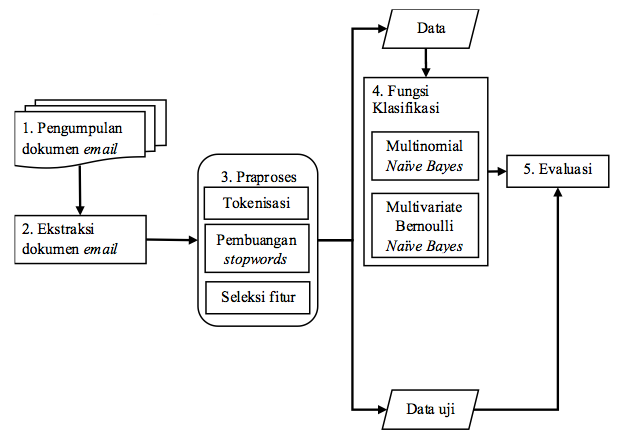
\includegraphics[width=400pt]{skemapenelitian.png}
	\caption{Diagram Alir Penelitian}
	\label{fig:skemapenelitian}
\end{figure*}

\subbab{Pengumpulan Dokumen Email}
Tahapan penelitian yang pertama adalah pengumpulan dokumen email. Dokumen email yang terkumpul digunakan sebagai korpus. Korpus yang digunakan pada penelitian ini adalah public email copus yang disediakan oleh Spamassasin\footnote{Diunduh dari  https://spamassassin.apache.org/publiccorpus/} dengan kode prefix “20030228”. Korpus email dibagi menjadi dua kelas yaitu kelas spam dan kelas ham. Korpus tersebut akan digunakan sebagai data latih dan data uji pada tahap selanjutnya.

\subbab{Ekstraksi Dokumen Email}
Dokumen email yang terdapat dalam korpus masih dengan format standar email yang terdiri dari header dan body. Oleh karena itu, struktur email tersebut harus dipecah sesuai dengan bagian-bagiannya. Ekstraksi dokumen email dilakukan untuk mendapatkan bagian email yang akan dimasukkan dalam proses tokenisasi. Tabel \ref{tab:strukturemail} menampilkan struktur yang terdapat dalam dokumen email. Bagian header yang digunakan untuk proses tokensisasi adalah subject, sedangkan pada bagian body adalah plain text dan HTML text.
\begin{table*}[h!]
	\begin{center}
		\caption{Struktur dokumen email}
		\label{tab:strukturemail}
		\small
		\begin{tabular}{l p{3cm} p{8cm}}
			\hline
			Bagian&Nama Struktur&Definisi\\
			\hline
			Header&MIME-version&Menunjukkan versi MIME yang digunakan\\
			&From&Nama dan alamat pengirim pesan\\
			&Received&Daftar semua server/komputer dimana pesan dapat sampai kepada penerimanya\\
			&Date&Menunjukkan tanggal dan waktu pesan email dibuat\\
			&Delivered-To&Alamat penerima email\\
			&Message-ID&Sebuah string unik yang diberikan oleh sistem mail saat pesan tersebut pertama kali dibuat\\
			&Subject To&Subjek dari pesan\\
			&To&Alamat yang mengirim pesan\\
			&X-Mailer&Aplikasi yang mengirimkan pesan\\
			&Return-Path&Alamat pengembalian pesan jika alamat penerima tidak ditemukan\\
			\hline
			Body&Plain text&Isi pesan dengan format penulisan dalam teks ASCII biasa\\
			&HTML text&Isi pesan yang mengandung tag HTML\\
			&Attachment&Informasi yang memberikan lampiran dari sebuah pesan\\
			\hline
		\end{tabular}
		\normalsize
	\end{center}
\end{table*}

\subbab{Praproses}
Dokumen email yang telah diekstraksi kemudian ditokenisasi. Tokenisasi adalah memotong dokumen teks menjadi potongan-potongan kecil yang disebut token dan membuang karakter-karakter tertentu seperti tanda baca (\cite{MANNING}). Whitespace (spasi, tab, newline) digunakan sebagai pemisah antar kata yang akan dipotong. Selain itu token yang dihasilkan biasanya diubah ke dalam bentuk lowercase. Proses tokensisasi dilakukan sebagai berikut:
\begin{itemize}
	\item Tanda baca diganti menjadi spasi sehingga tanda baca tersebut dianggap sebagai pemisah token. Tanda baca yang digunakan yaitu \'~- ) ( \textbackslash~ / = . , : ; ! ?.
	\item Teks dipotong menjadi token-token. Karakter numerik dibuang sehingga token hanya terdiri dari karakter huruf (string).
	\item Token dengan panjang kurang dari 3 karakter dibuang.
	\item Semua token diubah ke dalam bentuk lowercase.
\end{itemize}

Token yang termasuk ke dalam stopword\footnote{http://jmlr.org/papers/volume5/lewis04a/a11-smart-stop-list/english.stop} akan dibuang. Stopword adalah kata yang sangat umum dan sering muncul seperti kata sambung (\cite{MANNING}). Stopword tidak menambah informasi untuk fungsi klasifikasi dan untuk mengurangi beban komputasi.

Seleksi fitur merupakan suatu proses memilih subset dari setiap kata unik yang ada di dalam himpunan dokumen latih yang akan digunakan sebagai fitur di dalam klasifikasi dokumen. Subset kata unik yang terpilih disebut dengan penciri. Seleksi fitur memiliki dua tujuan, yaitu mengurangi jumlah kata yang digunakan dan meningkatkan akurasi hasil klasifikasi (\cite{MANNING}).

Pada penelitian ini, pemilihan fitur dilakukan dengan metode chi-square. Chi-square digunakan untuk menguji independensi antara dua kejadian yaitu kejadian kemunculan kata unik dan kejadian kemunculan kelas (\cite{MANNING}). Nilai chi-square kata t pada kelas c dihitung menggunakan persamaan:
\begin{equation}
	\label{eq:chisquare}
	\chi^2(t,c)=\sum_{e_t\in \{0,1\}}\sum_{e_c\in \{0,1\}}
	\frac{ [ N(e_te_c)-E(e_te_c) ]^2}{E(e_te_c)}
\end{equation}
\noindent dengan $N$ adalah frekuensi yang diamati dan $E$ adalah frekuensi yang diharapkan. Pada persamaan (\ref{eq:chisquare}), $e_t$ bernilai 1 jika dokumen mengandung kata $t$ dan $e_t$ bernilai 0 jika dokumen tidak mengandung kata $t$, sedangkan $e_c$ bernilai 1 jika dokumen terdapat dalam kelas $c$ dan $e_c$ bernilai 0 jika dokumen tidak terdapat dalam kelas $c$.
\begin{table*}[h!]
	\begin{center}
		\caption{Tabel kontingensi}
		\label{tab:kontingensi}
		\begin{tabular}{c c c}
			\hline
			\multirow{2}{*}{~~~~~Kata~~~~~}&\multicolumn{2}{c}{~~~~~~~~Kelas~~~~~~~~} \\
			\cline{2-3}
			&~~~$c$~~~&~~~$\neg c$~~~\\
			\hline
			$t$&A&B\\
			$\neg t$&C&D\\
			\hline
		\end{tabular}
	\end{center}
\end{table*}

Penghitungan nilai chi-square pada setiap kata $t$ yang muncul pada setiap kelas $c$ dapat dibantu dengan menggunakan tabel kontingensi (Tabel \ref{tab:kontingensi}). Nilai yang terdapat pada Tabel \ref{tab:kontingensi} merupakan nilai frekuensi obsevasi dari suatu kata terhadap kelas yaitu $A$ merupakan banyaknya dokumen pada kelas $c$ yang memuat kata $t$, $B$ merupakan banyaknya dokumen yang bukan kelas $c$ namun memuat kata $t$, $C$ merupakan banyaknya dokumen yang ada di kelas $c$ namun tidak memiliki kata $t$, serta $D$ merupakan banyaknya dokumen yang bukan kelas $c$ dan tidak memuat kata $t$.

Berdasarkan Tabel \ref{tab:kontingensi}, perhitungan chi-square pada (\ref{eq:chisquare}) dapat disederhanakan menjadi:
\begin{equation*}
	\label{eq:chisimple}
	\chi^2(t,c)=\frac{N(AD-BC)^2}{(A+C)(A+B)(B+D)(C+D)}
\end{equation*}
\noindent dengan $t$ merupakan kata yang diujikan terhadap suatu kelas $c$ dan $N$ merupakan jumlah dokumen latih.
\begin{table*}[h!]
	\begin{center}
		\caption{Nilai Kritis $\chi^2$}
		\label{tab:nilaikritis}
		\begin{tabular}{l r}
			\hline
			Taraf Nyata $(\alpha)$&Nilai Kritis\\
			\hline
			0.050&3.841\\ 
			0.025&5.024\\
			0.010&6.635\\
			0.005&7.879\\
			\hline
		\end{tabular}
	\end{center}
\end{table*}

Pengambilan keputusan dilakukan berdasarkan nilai $\chi^2$ dari masing-masing kata. Kata yang memiliki nilai $\chi^2$ lebih besar dari nilai kritis pada taraf nyata $\alpha$ adalah kata yang akan dipilih sebagai penciri dokumen. Kata yang dipilih sebagai penciri merupakan kata yang memiliki pengaruh terhadap kelas $c$. Nilai kritis $\chi^2$ untuk taraf nyata $\alpha$ (\cite{WALPOLE}) ditunjukkan pada Tabel \ref{tab:nilaikritis}.

Penelitian ini menggunakan satu taraf nyata $\alpha$ dengan nilai 0.01 yang diartikan bahwa kriteria kata yang dipilih sebagai penciri dokumen adalah kata yang memiliki nilai $\chi^2$ lebih besar dari 6.635. Hasil seleksi fitur ini akan digunakan sebagai vocabulary untuk proses klasifikasi.

\subbab{Fungsi Klasifikasi}
Ada dua cara mengelompokkan dokumen ke dalam kategori tertentu, yaitu manual dan otomatis. Cara pertama yaitu secara manual yang dilakukan oleh para pakar/ahli. Akan tetapi cara manual sulit dilakukan untuk dokumen dengan skala besar. Cara kedua adalah klasifikasi dokumen secara otomatis menggunakan fungsi klasifikasi yang dapat memetakan dokumen ke dalam kategori tertentu, $\gamma:\mathbb{X}\mapsto \mathbb{C}$, dengan $\mathbb{X}$ adalah kumpulan dokumen dan $\mathbb{C}$ adalah himpunan kelas atau kategori.

\citename{MANNING} membagi fungsi klasifikasi menjadi dua metode, yaitu metode berbasis vektor dan peluang. Pada fungsi klasifikasi berbasis vektor, setiap dokumen direpresentasikan sebagai vektor yang diberi label sesuai dengan kelasnya. Beberapa metode yang sering digunakan untuk klasifikasi berbasis vektor adalah kNN dan Rocchio classification.

Metode kedua adalah berbasis peluang dimana penentuan label kelas akan ditentukan dari nilai peluang dokumen terhadap kelas. Metode berbasis peluang yang sering digunakan adalah NB classifier. NB classifier terbagi menjadi dua model, yaitu Multivariate Bernoulli dan Multinomial NB.

Multivariate Bernoulli menyatakan bahwa dokumen diwakili oleh atribut biner yang menunjukkan ada dan tidak ada term dalam dokumen. Frekuensi kemunculan term dalam dokumen tidak ikut diperhitungkan. Ketika menghitung peluang dari sebuah dokumen, semua nilai atribut dikalikan termasuk kemungkinan ada dan tidak ada term dalam dokumen. Pada model ini, dokumen akan direpresentasikan ke dalam angka biner 1 jika terdapat dalam dokumen atau 0 jika tidak terdapat dalam dokumen:
\begin{equation*}
	d=<e_1, \dots, e_i, \dots e_M >, e_i\in \{0,1\}
\end{equation*}
\noindent Peluang dokumen $d$ dalam kelas $c$ dihitung menggunakan cara:
\begin{equation}
	\label{eq:peluangNBbernoulli}
	P(c|d)\propto \hat{P}(c)\prod_{t_i\in \mathbb{V}}\hat{P}(U_i=e_i|c)
\end{equation}
\noindent dengan $\hat{P}(U_i=e_i|c)$ adalah rasio dokumen dari kelas $c$ yang mengandung term $U_i$, $\hat{P}(c)$ adalah peluang dokumen pada kelas $c$. Pendugaan $\hat{P}(c)$ dan $\hat{P}(e_i|c)$ dihitung dengan cara:
\begin{equation*}
	\hat{P}(c)=\frac{N_c}{N},\xspace 
	\hat{P}(e_i|c)=\frac{T_{ct}}{\sum_{t\in V}T_{ct}}
\end{equation*}
\noindent dengan $T_{ct}$ adalah banyaknya dokumen yang mengandung term $t$ dalam dokumen latih kelas $c$. Untuk menghilangkan dugaan $\hat{P}(e_i|c)$ yang bernilai nol, digunakan Laplace smoothing atau Add-One Smoothing sehingga pendugaan $\hat{P}(e_i|c)$ menjadi:
\begin{equation}
	\label{eq:laplaceBernoulli}
	\hat{P}(e_i|c)=\frac{T_{ct}+1}{\sum_{t\in V}T_{ct}+b}
\end{equation}
\noindent dengan $b$ adalah banyaknya kelas atau kategori (\cite{MANNING}).

Dalam Multinomial NB, dokumen diwakili oleh serangkaian kemunculan term dari dokumen, yaitu:
\begin{equation*}
d=<t_1, \dots, t_k, \dots t_{n_d} >, t_k\in \mathbb{V}
\end{equation*}
\noindent Dalam model ini jumlah kemunculan dari setiap term dalam dokumen akan diperhitungkan. Peluang dokumen $d$ dalam kelas $c$ dihitung menggunakan persamaan:
\begin{equation}
\label{eq:peluangNBmultinom}
P(c|d)\propto \hat{P}(c)\prod_{1\leq k\leq n_d}\hat{P}(X=t_k|c)
\end{equation}
\noindent dengan $\hat{P}(X=t_k|c)$ adalah rasio term dalam kelas $c$ yang mengandung term $t$, $\hat{P}(c)$ adalah peluang dokumen pada kelas $c$. Pendugaan $\hat{P}(X=t_k|c)$ menggunakan Laplace smoothing yang dihitung dengan cara:
\begin{equation}
\label{eq:laplaceMultinom}
\hat{P}(t_k|c)=\frac{T_{ct}+1}{\sum_{t\in V}T_{ct}+b'}
\end{equation}
\noindent sedangkan $b'$ adalah banyaknya term dalam vocabulary.

\subbab{Evaluasi}
Langkah terakhir adalah melakukan pengujian dan evaluasi terhadap model klasifikasi yang telah dibuat. Pengujian dilakukan terhadap data uji yang telah ditentukan sebelumnya. Confussion Matrix (Tabel \ref{tab:confusionKelas}) digunakan untuk membantu perhitungan evaluasi dengan TP adalah banyaknya dokumen yang kelas aktualnya adalah kelas Spam dengan kelas prediksinya kelas Spam, FN adalah banyaknya dokumen yang kelas aktualnya adalah kelas Spam dengan kelas prediksinya kelas Ham, FP adalah banyaknya dokumen yang ada kelas aktualnya adalah kelas Ham dengan kelas prediksinya kelas Spam serta TN adalah banyaknya dokumen yang ada kelas aktualnya adalah kelas Ham dengan kelas prediksinya kelas Ham.
\begin{table*}[h!]
	\begin{center}
		\caption{Confussion Matrix kelas prediksi dan aktual}
		\label{tab:confusionKelas}
		\begin{tabular}{l c c}
			\hline
			\multirow{2}{*}{Kelas Aktual~~~~~~~~~~}&\multicolumn{2}{c}{Kelas Prediksi} \\
			\cline{2-3}
			&~~~~~Spam~~~~~&~~~~~Ham~~~~~\\
			\hline
			Spam&TP&FP\\
			Ham&FN&TN\\
			\hline
		\end{tabular}
	\end{center}
\end{table*}

\noindent Evaluasi penelitian ini menggunakan perhitungan akurasi dengan formula:
\begin{equation*}
	Akurasi=\frac{TP+TN}{TP+FN+FP+TN}
\end{equation*}

Untuk mengetahui akurasi setiap kelas digunakan perhitungan akurasi ham dan akurasi spam dengan formula:
\begin{equation*}
Akurasi~Ham=\frac{|H_k|}{|H|},~~Akurasi~Sam=\frac{|S_k|}{|S|}
\end{equation*}
\noindent dengan $|H_k|$ adalah banyaknya dokumen ham yang benar diklasifikasikan, $|H|$ adalah total dokumen ham, $|S_k|$ adalah banyaknya dokumen spam yang benar diklasifikasikan, dan $|S|$ adalah total dokumen spam.

Masing-masing model NB akan dihitung nilai akurasinya kemudian dibandingkan sehingga diketahui model mana yang paling baik untuk spam filter. Perbandingan model klasifikasi sebelum menggunakan seleksi fitur dan setelah menggunakan seleksi fitur dihitung untuk mengetaui pengaruh seleksi fitur terhadap model klasifikasi.

\subbab{Lingkungan Pengembangan}
Spesifikasi perangkat keras dan perangkat lunak yang digunakan untuk penelitian ini adalah sebagai berikut:
\begin{enumerate}
	\item Perangkat keras berupa komputer personal dengan spesifikasi sebagai berikut:
	\begin{itemize}
		\item Processor Intel Dual Core
		\item RAM 3GB
		\item Monitor LCD 14.0" HD
		\item Harddisk 250 GB HDD
	\end{itemize}
	\item Perangkat lunak:
	\begin{itemize}
		\item Sistem Operasi Windows 7
		\item Bahasa pemrograman PHP
		\item XAMPP v3.2.1
		\item Notepad++ digunakan sebagai editor kode program
	\end{itemize}
\end{enumerate}


	\bigskip
	\bigskip
	\bab{HASIL DAN PEMBAHASAN}
\subbab{Pengumpulan Dokumen Email}
Korpus yang digunakan pada penelitian ini adalah public email corpus yang disediakan oleh Spamassasin dengan kode prefix “20030228”. Korpus ini terdiri atas 6.047 pesan email yang sudah diklasifikasikan sebelumnya dengan komposisi:
\begin{itemize}
	\item 3900 easy-ham, yaitu pesan ham yang dapat dibedakan dengan mudah dari pesan spam karena tidak banyak mengandung ciri-ciri yang dimiliki oleh pesan spam.
	\item 250 hard-ham, yaitu pesan bertipe ham namun mengandung cukup banyak feature yang biasa terdapat pada pesan spam sehingga agak sulit diklasifikasikan.
	\item 1897 spam, yaitu pesan yang masuk dalam kategori spam.
\end{itemize}

Dari masing-masing kategori, secara acak diambil sebanyak 70\% sebagai data latih dan sisanya digunakan data uji. Pesan yang memiliki label easy-ham dan hard-ham digabungkan ke dalam satu kategori yaitu ham. Dengan demikian, dokumen email tersebut diklasifikasikan ke dalam dua kategori yaitu spam dan ham dengan komposisi:
\begin{itemize}
	\item Total dokumen ham 4150, sebanyak 2905 dokumen digunakan sebagai data latih dan 1245 dokumen digunakan sebagai data uji.
	\item Total dokumen spam 1897, sebanyak 1328 dokumen digunakan sebagai data latih dan 569 dokumen digunakan sebagai data uji.
\end{itemize}

Hasil pengamatan menunjukkan dokumen spam rata-rata mempunyai ukuran data yang lebih besar dibandingkan dengan dokumen ham. Ukuran terbesar dari dokumen ham adalah 301 KB, sedangkan untuk dokumen spam adalah 232 KB. Besar ukuran dokumen email tergatung dari isi yang terdapat di dalam dokumen. Dokumen email dengan content-type multipart biasanya menghasilkan ukuran data yang lebih besar dibandingkan dengan singlepart.

\subbab{Ekstraksi Dokumen Email}
Langkah ekstraksi dokumen dilakukan untuk memecah dokumen email menjadi bagian-bagian yang lebih kecil. Langkah ini diperlukan karena tidak semua bagian email digunakan untuk tahapan selanjutnya. Struktur header seperti sender, return path, dan X-mailer hanya muncul pada beberapa dokumen email sehingga tidak bagus digunakan sebagai penciri. Subject email merupakan salah satu bagian email yang baik digunakan sebagai penciri (\cite{SAHAMI}). Bagian struktur email yang digunakan untuk langkah selanjutnya adalah subject dan body (plain text dan HTML text).

Ekstraksi dokumen menggunakan library mailparse\footnote{Dapat diunduh pada http://pecl.php.net/package/mailparse} yang telah tersedia untuk bahasa pemrograman php. Hasil pengamatan menunjukkan content plain text paling banyak ditemukan pada dokumen easy-ham, sedangkan HTML text banyak ditemukan pada dokumen hard-ham dan spam.

\subbab{Praproses}
Tahap tokenisasi dilakukan pada bagian email yang digunakan. Dalam tahap tokenisasi data latih diperoleh 67612 token. Seluruh token tersebut disaring dengan membuang kata-kata yang terdapat dalam daftar stopword sehingga diperoleh token sebanyak 67172. Dapat disimpulkan bahwa hanya sebanyak 0.7\% dari seluruh token data latih merupakan stopword. Dengan menggunakan seleksi fitur chi-square dan taraf $\alpha$ = 0.01, token akhir yang dijadikan sebagai vocabulary adalah 3866 token atau 5.8\% dari total token setelah pembuangan stopword. Tabel \ref{tab:jumlahToken} menunjukkan jumlah token yang dihasilkan pada setiap langkah praproses. Sebanyak 2273 token terdapat pada kelas ham dan spam seperti kata “absolutely”, “account” dan “address” termasuk tag-tag HTML. Sedangkan sebanyak 690 token hanya terdapat pada kelas ham dan 882 token hanya terdapat pada kelas spam. Gambar \ref{fig:komposisitoken} menunjukkan komposisi jumlah token terhadap kelas dari hasil seleksi fitur.
\begin{table*}[h!]
	\begin{center}
		\caption{Jumlah token yang dihasilkan}
		\label{tab:jumlahToken}
		\begin{tabular}{l r}
			\hline
			Tahapan~~~~~~~~~~&~~~~~~~~~~Jumlah Token \\
			\hline
			Tokenisasi &67612\\
			Membuang Stopword &67172\\
			Seleksi Fitur&3866\\
			\hline
		\end{tabular}
	\end{center}
\end{table*}
\begin{figure*}[h!]
	\centering
	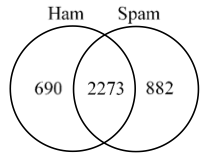
\includegraphics[width=130pt]{hamspam.png}
	\caption{Komposisi jumlah token hasil tahap seleksi fitur}
	\label{fig:komposisitoken}
\end{figure*}

\subbab{Fungsi Klasifikasi Naive Bayes}
Setelah melewati langkah praproses, langkah selanjutnya adalah membuat fungsi klasifikasi yang dapat memetakan dokumen ke dalam kategori tertentu. Pada model Multivariate Bernoulli, pendugaan parameter setiap term dihitung menggunakan persamaan (\ref{eq:peluangNBbernoulli}). Peluang dari pendugaan parameter Multivariate Bernoulli bergantung pada nilai document frequency (DF). Semakin besar nilai DF maka semakin besar pula peluangnya. Tabel 6 menunjukkan lima term urutan tertinggi hasil pendugaan parameter Multivariate Bernoulli berdasar pada nilai DF dan peluangnya. Tabel \ref{tab:limaTermMultivar} menunjukkan pada kelas ham, jika dibandingkan term ‘listinfo’ yang bernilai DF 1839 menghasilkan peluang sebesar 0.633, sedangkan untuk term ‘wrote’ dengan nilai DF 1230 menghasilkan peluang yang lebih kecil yaitu sebesar 0.423.
\begin{table*}[h!]
	\begin{center}
		\caption{Lima term hasil pendugaan pada Multivariate Bernoulli}
		\label{tab:limaTermMultivar}
		\begin{tabular}{l r r | l r r}
			\hline
			\multicolumn{3}{c|}{Kelas Ham}&\multicolumn{3}{c}{Kelas Spam}\\
			\hline
			Term&DF&Peluang&Term&DF&Peluang\\
			\hline
			listinfo&1839&0.633&html&758&0.571\\
			list&1619&0.558&email&729&0.549\\
			mailman&1617&0.557&click&721&0.543\\
			www&1611&0.555&href&690&0.520\\
			wrote&1230&0.423&body&671&0.505\\
			\hline
		\end{tabular}
	\end{center}
\end{table*}

Pada model Multinomial NB, pendugaan parameter dihitung menggunakan persamaan (\ref{eq:peluangNBmultinom}). Berbeda dengan model Multivariate Bernoulli, nilai peluang model Multinomial NB dipengaruhi oleh nilai TF (term frequency). Semakin tinggi nilai TF maka semakin besar pula peluangnya. Tabel \ref{tab:limaTermMultinom} menunjukkan lima term urutan tertinggi hasil pendugaan parameter Multinomial NB berdasar pada nilai TF dan peluangnya. Tabel \ref{tab:limaTermMultinom} menunjukkan pada kelas ham, jika dibandingkan term ‘width yang bernilai TF 16815 menghasilkan peluang sebesar 0.038, sedangkan untuk term ‘src’ dengan nilai TF 9340 menghasilkan peluang yang lebih kecil yaitu sebesar 0.021. Pendugaan $\hat{P}(c)$ untuk setiap model bernilai sama yaitu $\hat{P}(ham)$=0.686 sedangkan $\hat{P}(spam)$=0.314.
\begin{table*}[h!]
	\begin{center}
		\caption{Lima term hasil pendugaan pada Multinomial NB}
		\label{tab:limaTermMultinom}
		\begin{tabular}{l r r | l r r}
			\hline
			\multicolumn{3}{c|}{Kelas Ham}&\multicolumn{3}{c}{Kelas Spam}\\
			\hline
			Term&TF&Peluang&Term&TF&Peluang\\
			\hline
		width&16815&0.038&font&27602&0.090\\
		www&12055&0.027&size&10335&0.033\\
		font&11042&0.025&width&7855&0.025\\
		height&9598&0.022&color&7892&0.025\\
		src&9340&0.021&face&7594&0.024\\
			\hline
		\end{tabular}
	\end{center}
\end{table*}

\subbab{Evaluasi}
Proses pengujian model klasifikasi dilakukan menggunakan
yang terdiri dari 1245 dokumen ham dan 569 dokumen spam. Pengujian menggunakan pendugaan parameter yang telah dibuat pada tahap fungsi klasifikasi. Persamaan (\ref{eq:peluangNBbernoulli}) digunakan pada pengujian model Multivariate Bernoulli sedangkan (\ref{eq:peluangNBmultinom}) digunakan untuk menguji model Multinomial NB. Perhitungan (\ref{eq:peluangNBbernoulli}) dan (\ref{eq:peluangNBmultinom}) menghasilkan nilai 0 karena nilai peluang yang dihasilkan sangat kecil. Oleh karena itu, untuk mengatasi hal tersebut semua nilai pendugaan parameter dijadikan log sehingga persamaan (\ref{eq:peluangNBbernoulli}) menjadi:
\begin{equation*}
\log(P(c|d))\propto \log(\hat{P}(c))+\sum_{t_i\in \mathbb{V}}\log(\hat{P}(U_i=e_i|c))
\end{equation*}
\noindent sedangkan persamaan (\ref{eq:peluangNBmultinom}) menjadi:
\begin{equation*}
\log(P(c|d))\propto \log(\hat{P}(c))+\sum_{1\leq k\leq n_d}\log(\hat{P}(X=t_k|c))
\end{equation*}

Pada semua dokumen uji dilakukan pengujian terhadap setiap model klasifikasi baik sebelum dan sesudah menggunakan seleksi fitur chi-square. Hasil pengujian dalam bentuk confussion matrix terdapat pada lampiran 1. Akurasi tertinggi dicapai model Multinomial NB tanpa seleksi fitur chi-square dengan tingkat akurasi sebesar 95.31\%. Model Multivariate Bernoulli tanpa seleksi fitur chi-square memiliki tingkat akurasi terendah yaitu sebesar 89.69\%. Secara keseluruhan, model Multinomial NB menunjukkan tingkat akurasi yang lebih tinggi, baik menggunakan seleksi fitur atau tidak. Gambar \ref{fig:akurasimodel} menunjukkan tingkat akurasi dari model klasifikasi yang telah dibuat.
\begin{figure*}[h!]
	\centering
	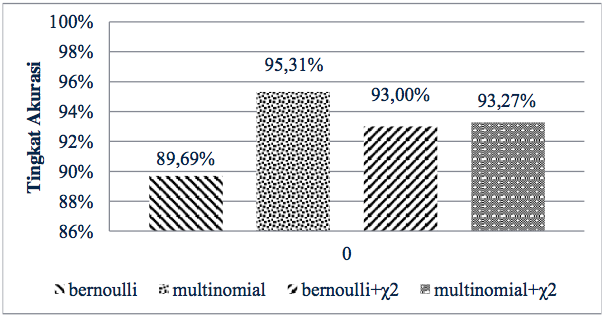
\includegraphics[width=400pt]{akurasimodel.png}
	\caption{Tingkat akurasi setiap model klasifikasi}
	\label{fig:akurasimodel}
\end{figure*}

Gambar \ref{fig:seleksifitur} menunjukkan pengaruh dari seleksi fitur terhadap model klasifikasi. Dengan menggunakan seleksi fitur chi-square, terjadi penuruan akurasi sebesar 1.98\% pada model Multinomial NB. Hal ini berbanding terbalik pada model Multivariate Bernoulli yang mengalami peningkatan akurasi sebesar 3.31\%. Banyaknya vocabulary yang digunakan mempengaruhi turun-naiknya akurasi model klasifikasi. Multivariate Bernoulli lebih baik jika vocabulary yang digunakan berjumlah sedikit, sedangkan untuk vocabulary dalam jumlah banyak, Multinomial NB menghasilkan tingkat akurasi yang lebih baik.
\begin{figure*}[h!]
	\centering
	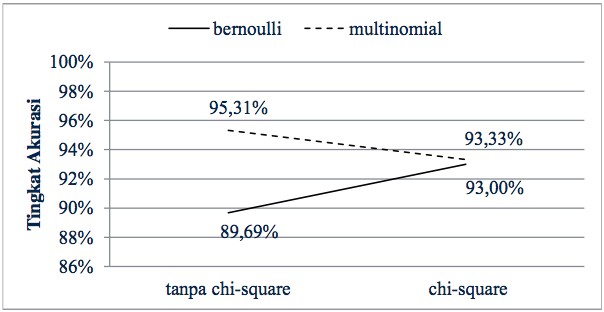
\includegraphics[width=400pt]{seleksifitur.png}
	\caption{Pengaruh seleksi fitur terhadap model klasifikasi}
	\label{fig:seleksifitur}
\end{figure*}
\begin{figure*}[h!]
	\centering
	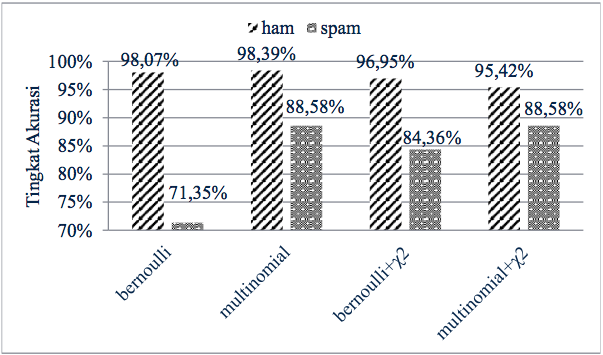
\includegraphics[width=400pt]{akurasihamspam.png}
	\caption{Tingkat akurasi ham dan spam setiap model klasifikasi}
	\label{fig:akurasihamspam}
\end{figure*}

Model Multinomial NB tanpa seleksi fitur chi-square sangat baik dalam mengenali dokumen ham dengan tingkat akurasi 98.39\%. Sedangkan dalam mengenali dokumen spam, model Multinomial NB dengan seleksi fitur chi-square dan tanpa seleksi fitur sama-sama menghasilkan akurasi yang terbaik yaitu sebesar 88.58\%. Gambar \ref{fig:akurasihamspam} menunjukkan tingkat akurasi ham dan spam setiap model klasifikasi. Setiap model klasifikasi menunjukkan tingkat akurasi ham selalu lebih baik dibandingkan dengan akurasi spam.


	\bigskip
	\bigskip
	\bab{SIMPULAN DAN SARAN}
\subbab{Simpulan}
Berdasarkan penelitian yang telah dilakukan, dapat disimpulkan beberapa hal sebagai berikut:
\begin{enumerate}
	\item Model Multinomial NB tanpa seleksi fitur chi-square menghasilkan akurasi tertinggi sebesar 95.31\%, sedangkan untuk tingkat akurasi terendah didapatkan pada model Multivariate Bernoulli tanpa seleksi fitur chi-square dengan akurasi sebesar 89.69\%.
	\item Seleksi fitur chi-square mempengaruhi tingkat akurasi model klasifikasi. Seleksi fitur chi-square meningkatkan akurasi model Multivariate Bernoulli sebesar 3.31\%, sedangkan Multinomial NB mengalami penurunan akurasi sebesar 1.98\%.
	\item Dari semua pengujian, pengenalan dokumen ham selalu lebih baik dibandingkan dengan pengenalan dokumen spam.
	\item Secara keseluruhan model Multinomial NB menghasilkan akurasi yang lebih baik dibandingkan dengan model Multivariate Bernoulli.
\end{enumerate}

\subbab{Saran}
Pada penelitian ini, pengenalan dokumen ham menghasilkan akurasi yang tinggi, tetapi pengenalan spam menghasilkan akurasi yang rendah. Dengan menggunakan model klasifikasi berbasis aturan, dokumen spam sulit diklasifikasikan karena penciri antara dokumen ham dan spam banyak mempunyai kemiripan. Spam email mempunyai beberapa penciri yang unik dan dapat mudah diklasifikasikan tanpa perhitungan peluang. Penggabungan model klasifikasi Naive Bayes dan model klasifikasi berbasis aturan (hand-crafted rules) diharapkan dapat meningkatkan akurasi pada pengenalan dokumen spam sehingga pada penelitian selanjutnya kinerja spam filter dapat lebih baik.

	
	\renewcommand{\bibname}{DAFTAR PUSTAKA}
	\bigskip
	\bigskip
	\xpatchbibmacro{date+extrayear}{%
			\printtext[parens]%
		}{%
		\setunit{\addperiod\space}%
		\printtext%
	}{}{}
	\sloppy
	\addcontentsline{toc}{chapter}{DAFTAR PUSTAKA}
	\printbibliography

	\pagebreak
	\appendix
	\label{lamp:lampiran}
	\chaptermark{LAMPIRAN}
	\addcontentsline{toc}{chapter}{LAMPIRAN}
	%% -----------------------------------
%% CONTOH LAMPIRAN 1
%%
\lampiran{Confussion Matrix untuk setiap pengujian model klasifikasi} 
\label{lamp:confusionmatrix}
\begin{table*}[h!]
	\begin{center}
		\begin{tabular}{l l r r}
			\hline
			\multirow{2}{*}{Model}&\multirow{2}{*}{Kelas Aktual}&\multicolumn{2}{c}{Kelas Prediksi}\\
			\cline{3-4}
			&&~~~~~Spam&~~~~~$\neg$Spam\\
			\hline
			~&~&~&\\
			Multivariate Bernoulli tanpa $\chi^2$&Spam&406&163\\
			&$\neg$Spam&24&1221\\
			~&~&~&\\
			\hline
			~&~&~&\\
			Multivariate NB tanpa $\chi^2$&Spam&504&65\\
			&$\neg$Spam&20&1225\\
			~&~&~&\\
			\hline
			~&~&~&\\
			Multivariate Bernoulli dengan $\chi^2$&Spam&480&89\\
			&$\neg$Spam&38&1207\\
			~&~&~&\\
			\hline
			~&~&~&\\
			Multivariate NB dengan $\chi^2$&Spam&504&65\\
			&$\neg$Spam&57&1188\\
			~&~&~&\\
			\hline	
		\end{tabular}
	\end{center}
\end{table*}
\pagebreak
%% -----------------------------------
%% CONTOH LAMPIRAN 2
%%
\lampiran{Algoritme ukuran kesamaan antar dokumen} 
\label{lamp:kesamaandokumen}

\pagebreak
	\bab{RIWAYAT HIDUP}
Penulis dilahirkan di Sumedang pada tanggal 8 Juni 1990 dari ayah Dedi Kusnadi dan ibu Ai Sumartini. Penulis adalah putra kedua dari tiga bersaudara. Tahun 2008 penulis lulus SMA Negeri 1 Sumedang dan pada tahun yang sama penulis lulus seleksi masuk Institut Pertanian Bogor Program Diploma, Program Keahlian Manajemen Informatika. Setelah menempuh pendidikan pada program Diploma penulis melanjutkan pendidikan tingkat sarjana pada program Ekstensi Ilmu Komputer IPB angkatan ke-7.

	\endgroup	
	
%----------------------------------------------------------------
\end{document}